%!TEX root = ../tesis.tex
\section{Métodos de Interpolación}
\label{sec:identificacion-focos-interpolacion}
Todos los métodos de interpolación se basan en la presunción lógica de que
cuanto más cercanos están dos puntos sobre la superficie terrestre, los
valores de cualquier variable cuantitativa que midamos en ellos serán más
parecidos, para expresarlo más técnicamente, las variables espaciales
muestran autocorrelación espacial[2].

La interpolación espacial, consiste en usar puntos con valores conocidos,
también llamados puntos de control, para estimar una variable en lugares
donde se desconoce; también se considera una forma de transformar información
puntual en información de superficie, con el objetivo de combinarla con
otros datos para facilitar el análisis y la modelación espacial.
El resultado de la interpolación espacial depende de un algoritmo
computacional o una ecuación matemática en la cual se emplean los datos
de los puntos de control[1].

\section{Métodos de interpolación locales}
Los método locales, utilizan la interpolación utilizando la información
de los puntos más cercanos. Asumen autocorrelación espacial y estiman los
valores de Z como una media ponderada de los valores de un conjunto de
puntos de muestreo cercanos[2].

\subsection{Polígonos de Voronoi}
Es uno de los métodos de interpolación más simples, simples basado en la
distancia euclidiana. Se crean al unir los puntos entre sí, trazando las
mediatrices de los segmento de unión. Las intersecciones de estas mediatrices
determinan una serie de polígonos en un espacio bidimensional alrededor de
los puntos de control, de manera que el perímetro de los polígonos generados
sea equidistante a los puntos vecinos y designando su área de influencia, como :
\begin{itemize}
    \item Centros hospitalarios.
    \item Estaciones de bomberos.
    \item Bocas de metro.
    \item Centros comerciales.
    \item Control del tráfico aéreo.
    \item Telefonía móvil.
\end{itemize}

\subsection{Ponderación de la inversa de la distancia (IDW)}
Estima los puntos del modelo realizando una asignación de pesos a los datos
del entorno en función inversa a la distancia que los separa del punto en
cuestión. De esta forma, se acepta  que  los puntos más próximos al centroide
intervienen de manera más relevante en la obtención del valor definitivo
de Z para ese punto.

La elección del exponente de ponderación(p) determina la contribución de
los puntos circundantes al punto problema, cuanto mayor es p, más contribuyen
los puntos próximos. Es necesario contar con muchos puntos para la interpolación.

Uno de los problemas más importantes de los métodos basados en medias
ponderadas es que, interpolan basándose en el valor medio de un conjunto
de puntos situados en las proximidades, por tanto nunca se van a obtener
valores mayores o menores que los de los puntos utilizados para hacer la
interpolación[2]. En consecuencia no se van a interpolar correctamente
máximos o mínimos locales y además los puntos de muestreo aparecen en el
mapa final como máximos y mínimos locales erróneos.

\subsection{Kriging}
El Kriging es un método geoestadístico de interpolación espacial de carácter
global, exacto y estocástico. La idea básica de este método corresponde a
la noción de dependencia espacial, según la cual las muestras cercanas
tienen mayor similitud entre sí que las más apartadas[1].

Se presenta con un método de interpolación con una expresión general
similar a la anterior (IDW). La diferencia básica es que asume que la
altitud puede definirse como una variable regionalizada. Supone que la
variación espacial de la variable a representar puede ser explicada al
menos parcialmente mediante funciones de correlación espacial(la variación
espacial de los valores de z puede deducirse de los valores circundantes
de acuerdo con unas funciones homogéneas en toda el área) [4].

\subsection{Tipos de Kriging}
Kriging simples
Asume que las medias locales son relativamente constantes y de valor muy
semejante a la media de la población que es conocida. La media de la
población es utilizada para cada estimación local, en conjunto con los
puntos vecinos establecidos como necesarios para la estimación.
Kriging ordinario
Las medias locales no son necesariamente próximas de la media de la población,
usándose apenas los puntos vecinos para la estimación. Es el método más
ampliamente utilizado en los problemas ambientales.

\subsection{Semivarianza y semivariograma}
El método de Kriging utiliza diversas teorías explayadas en la estadística.
Una semivarianza es la medida del grado de dependencia espacial entre dos
muestras. La magnitud de la semivarianza entre dos puntos depende de la
distancia entre ellos. Efecto pepita,  es el valor del semivariograma en
el origen. Resulta del componente aleatorio, no correlacionado espacialmente,
que experimenta cualquier variable espacial. Se denomina así por las pepitas
de oro que representan un brusco incremento en la variable concentración de
oro para distancias muy cortas.
Meseta, es el valor máximo que adopta el semivariograma para distancias
elevadas más allá de las cuales no hay autocorrelación espacial.
Rango, es la distancia a la que se alcanza la meseta. Puede asimilarse a
la distancia más allá de la cual dos medidas pueden considerarse independientes.


\section{Identificación de los focos de dengue}
\label{sec:solucion-instantanea}
%~ %~
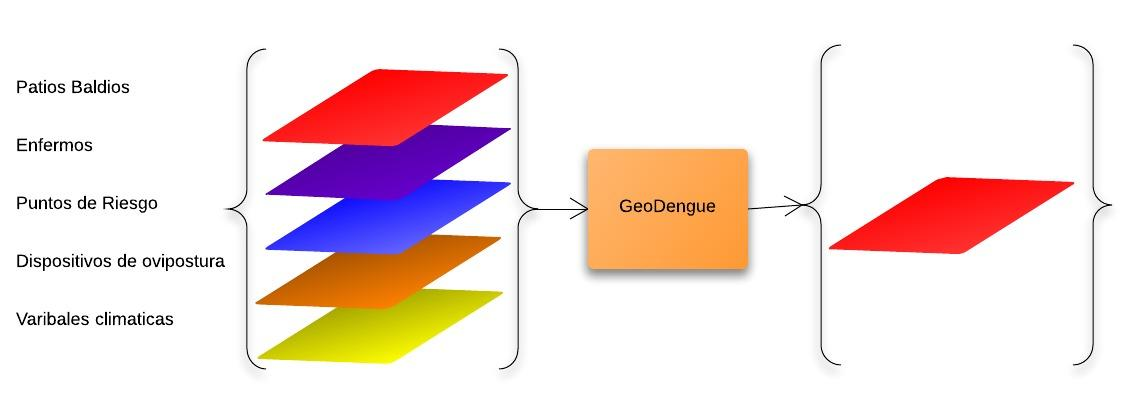
\includegraphics[ scale=0.35]{./graphics/modelo-base.jpeg}
%~ %~
Mediante técnicas de interpolación espacial los datos de entrada serán
procesados y representados en la zona de estudio como polígonos que
representan focos de la enfermedad.
%~ %~
Los focos se determina según los valores conocidos de las larvitrampas
mediante interpolación, esto representa un instante \cite{AnusuyaSpeech2009}.
